\section{矩阵分析及其应用}

\subsection{矩阵序列与矩阵级数}

\begin{definition}[矩阵序列的收敛]
设有矩阵序列 $\{A^{(k)}=(a_{ij}^{(k)})\}$,若各分量分别收敛,则称 $\{A^{(k)}\}$ 收敛;否则,若存在一组 $i,j$ 使得 $a_{ij}^{(k)}$ 发散,则称 $\{A^{(k)}\}$ 发散。
\end{definition}

\begin{theorem}[各分量收敛等价于依范数收敛]
设 $A^{(k)}\in\mathbb C^{m\times n}$,$\norm{\cdot}$ 为任一\textbf{广义矩阵范数},则:
\begin{align*}
    &A^{(k)}\to 0\iff \norm{A^{(k)}}\to 0\\
    &A^{(k)}\to A\iff \norm{A^{(k)}-A}\to 0
\end{align*}
\end{theorem}
\begin{proof}
根据广义矩阵范数的等价性定理,仅需对 $m_\infty$ 范数证明。由于:
\[
    a^{(k)}\to 0\wedge b^{(k)}\to 0\iff\max(a^{(k)},b^{(k)})\to0
\]
所以:
\[
    A^{(k)}\to 0\iff |a_{ij}^{(k)}|\to 0\iff\norm{A}_{m_\infty}=\max_{i,j}|a_{ij}^{(k)}|\to 0
\]
\end{proof}

\begin{remark}
按各元素收敛需要验证 $m\times n$ 个数列是否收敛,比较麻烦;而依范数收敛只需要验证 1 个数列是否收敛,更加方便。
\end{remark}

\begin{remark}
尽管上述定理对任意\textbf{广义矩阵范数}都成立,但在证明时我们通常会选取一个\textbf{矩阵范数},这样可以用上\textbf{相容性条件},使得很多证明与高等数学中证明数列收敛没有什么区别。
\end{remark}

\begin{definition}[Cauchy 收敛]
矩阵序列 $\{A^{(k)}\}$ 收敛的充要条件是:对任意 $\epsilon>0$,存在 $N(\epsilon)$,当 $k,l\geq N(\epsilon)$ 时,有:
\[
    \norm{A^{(k)}-A^{(l)}}<\epsilon
\]
其中 $\norm\cdot$ 为任一广义矩阵范数。
\end{definition}

\begin{remark}
站在更高的泛函分析的角度,由于所有有限维赋范空间都是完备的,所以 Cauchy 列必收敛。
\end{remark}

\begin{property}
若 $A^{(k)}\to A$,则 $\norm{A^{(k)}}\to\norm{A}$.
\end{property}
\begin{proof}
\[
    \left|\norm{A^{(k)}}-\norm{A}\right|\leq\norm{A^{(k)}-A}\to0\implies\norm{A^{(k)}}\to\norm{A}
\]
\end{proof}

\begin{property}
设 $A^{(k)}\to A,\,B^{(k)}\to B$,则:
\begin{align*}
    &\lim_{k\to\infty}\left(\alpha A^{(k)}+\beta B^{(k)}\right)=\alpha A+\beta B\\
    &\lim_{k\to\infty}A^{(k)}B^{(k)}=AB
\end{align*}
\end{property}
\begin{proof}
只考虑相容的矩阵范数。
\begin{align*}
    \norm{A^{(k)}B^{(k)}-AB}&=\norm{A^{(k)}B^{(k)}-AB^{(k)}+AB^{(k)}-AB}\\
    &\leq\norm{A^{(k)}B^{(k)}-AB^{(k)}}+\norm{AB^{(k)}-AB}\\
    &\leq\norm{A^{(k)}-A}\norm{B^{(k)}}+\norm{A}\norm{B^{(k)}-B}
\end{align*}
由于 $\norm{A^{(k)}-A}\to0,\,\norm{B^{(k)}}\to\norm B,\,\norm{B^{(k)}-B}\to0$,所以 $\norm{A^{(k)}B^{(k)}-AB}\to0$,故 $A^{(k)}B^{(k)}\to AB$.
\end{proof}

\begin{theorem}
$A^{(k)}\to A$ 的充要条件是对任意 $x$ 有 $A^{(k)}x\to Ax$,或者对任意 $x,y$ 有 $y^HA^{(k)}x\to y^HAx$.
\end{theorem}

\begin{theorem}
若 $A^{(k)}$ 和 $A$ 都为 Hermite 矩阵,那么 $A^{(k)}\to A$ 的充要条件是 $x^HA^{(k)}x=x^HAx,\forall x$.
\end{theorem}

\begin{corollary}[类比单调有界定理]
若 $A^{(k)}$ 为半正定 Hermite 矩阵且单调减少(即 $A^{(k)}-A^{(k+1)}$ 为半正定 Hermite 矩阵),那么 $A^{(k)}$ 有极限。
\end{corollary}

\begin{property}
设 $A^{(k)}\to A$,且 $A^{(k)}$ 和 $A$ 都可逆,则:
\[
    \lim_{k\to\infty}\left(A^{(k)}\right)^{-1}=A^{-1}
\]
\end{property}

\begin{definition}[有界]
如果存在常数 $M>0$,使得对所有 $k$ 都有:
\[
    |a_{ij}^{(k)}|<M
\]
或等价地:
\[
    \norm{A^{(k)}}<M^\ast
\]
则称矩阵序列 $\{A^{(k)}\}$ 为有界的。
\end{definition}

\begin{theorem}
有界矩阵序列 $\{A^{(k)}\}$ 一定有收敛的子列。
\end{theorem}

\begin{definition}[收敛矩阵]
设 $A$ 为方阵且 $A^k\to 0\,(k\to\infty)$,则称 $A$ 为收敛矩阵。
\end{definition}

\begin{theorem}[迭代法基本定理]
\label{thm:iterbase}
$A$ 是收敛矩阵的充要条件是 $\rho(A)<1$.
\end{theorem}
\begin{proof}
必要性:设 $\lambda,x$ 为 $A$ 的特征值和特征向量,$\lambda x=Ax$,则 $\lambda^kx=A^kx$.  两边取范数:
\[
    |\lambda|^k\norm{x}=\norm{A^kx}\leq\norm{A^k}\norm{x}	
\]
由于 $x\neq 0$,故 $|\lambda|^k\leq\norm{A^k}\to0\,(k\to\infty)$,于是 $|\lambda|<1$,故 $\rho(A)=\max_i|\lambda_i|<1$.

充分性:取 $\epsilon=(1-\rho(A))/2$,根据定理 \ref{thm:specrad-norm},存在某种矩阵范数使得:
\[
    \norm{A}<\rho(A)+\epsilon<1
\]
故:
\[
    \norm{A^k}\leq\norm{A}^k<(\rho(A)+\epsilon)^k\to 0\quad(k\to\infty)
\]
从而 $A^k\to0$.
\end{proof}

\begin{theorem}
$A$ 是收敛矩阵的充要条件是存在某种矩阵范数满足 $\norm{A}<1$.
\end{theorem}
\begin{proof}
根据迭代法基本定理和谱半径与矩阵范数的关系易证。
\end{proof}

\begin{remark}
实际应用中不会去算 $\rho(A)$(解特征值很麻烦),而是计算 $\norm{A}$.
\end{remark}

\begin{example}
在\textbf{迭代法解线性方程组}中,设迭代格式为 $x_{n+1}=Ax_n+f$,则:
\begin{align*}
    x_{n}&=Ax_{n-1}+f\\
    &=A^2x_{n-2}+Af+f\\
    &=\cdots\\
    &=A^n x_0+(A^{n-1}+\cdots+A+I)f\\
    &=A^n x_0+(I-A^n)(I-A)^{-1}f\\
    &=A^nx_0+(I-A)^{-1}f-A^n(I-A)^{-1}f
\end{align*}
若迭代收敛,则解满足 $x=Ax+f\implies x=(I-A)^{-1}f$.  记 $\epsilon_n=x_n-x$ 表示第 $n$ 次迭代后的误差,$\epsilon_0=x_0-x$ 表示初始误差,那么:
\[
\epsilon_n=A^n\epsilon_0
\]
因此,当 $A$ 是收敛矩阵时,$\epsilon_n\to0$,迭代法收敛。
\end{example}

\begin{definition}[矩阵级数的收敛与绝对收敛]
称矩阵级数 $\sum_{k=0}^\infty A^{(k)}$ (绝对)收敛到 $S$,若其部分和序列 $\left\{S_N=\sum_{k=0}^N A^{(k)}\right\}$ (绝对)收敛,且极限为 $S$.
\end{definition}

\begin{property}
矩阵级数 $\sum_{k=0}^\infty A^{(k)}$ 收敛的充要条件是对任意向量 $x$,向量级数 $\sum_{k=0}^\infty A^{(k)}x$ 收敛。
\end{property}

\begin{property}
若矩阵级数是绝对收敛的,则它一定是收敛的,并且任意调换其项的顺序所得到的级数仍然是收敛的,且其和不变。
\end{property}

\begin{property}
矩阵级数 $\sum_{k=0}^\infty A^{(k)}$ 绝对收敛的充要条件是 $\sum_{k=0}^\infty\norm{A^{(k)}}$ 收敛。
\end{property}

\begin{property}
若矩阵级数 $\sum_{k=0}^\infty A^{(k)}$ (绝对)收敛,则 $\sum_{k=0}^\infty PA^{(k)}Q$ 也(绝对)收敛,且:
\[
    \sum_{k=0}^\infty PA^{(k)}Q=P\left(\sum_{k=0}^\infty A^{(k)}\right)Q
\]
\end{property}

\begin{property}
若两个矩阵级数都绝对收敛,且分别收敛到 $A,B$,则其 Cauchy 乘积 $\sum_{k=0}^\infty\sum_{i+j=k}A^{(i)}B^{(j)}$ 绝对收敛,且收敛到 $AB$.
\end{property}

\begin{theorem}
方阵 $A$ 的幂级数 $\sum_{k=0}^\infty A^k$ 收敛的充要条件是 $\rho(A)<1$,且收敛时的和为 $(I-A)^{-1}$.
\end{theorem}
\begin{proof}
必要性。由于级数 $I+A+A^2+\cdots$ 收敛,所以部分和序列 $S^{(k)}=I+A+\cdots+A^k$ 收敛。记 $T^{(k)}=I+A+\cdots+A^{k+1}$,则 $A^{k+1}=T^k-S^k\to0$,即 $A$ 是收敛矩阵。根据定理 \ref{thm:iterbase},有 $\rho(A)<1$.

充分性。已知 $\rho(A)<1$,故 $A$ 为收敛矩阵,$A^k\to 0$.  于是 $S^{(k)}=I+A+\cdots+A^k=(I-A)^{-1}-(I-A)^{-1}A^{k+1}\to(I-A)^{-1}$.
\end{proof}

\begin{theorem}
若方阵 $A$ 的某一范数满足 $\norm{A}<1$,则部分和 $I+A+\cdots+A^N$ 与 $(I-A)^{-1}$ 之间的误差为:
\[
    \left\Vert(I-A)^{-1}-\sum_{k=0}^NA^k\right\Vert\leq\frac{\norm{A}^{N+1}}{1-\norm{A}}
\]
\end{theorem}
\begin{proof}
设 $B=(I-A)^{-1}-\sum_{k=0}^NA^k=(I-A)^{-1}A^{N+1}$,则 $(I-A)B=A^{N+1}$,即 $B=AB+A^{N+1}$,从而:
\[
    \norm{B}=\norm{AB+A^{N+1}}\leq\norm{A}\norm{B}+\norm{A}^{N+1}\implies\norm{B}\leq\frac{\norm{A}^{N+1}}{1-\norm{A}}
\]
\end{proof}

\begin{theorem}
设幂级数 $\sum_{k=0}^\infty c_kz^k$ 的收敛半径为 $r$,如果方阵 $A$ 满足 $\rho(A)<r$,则矩阵幂级数 $\sum_{k=0}^\infty c_kA^k$ 绝对收敛;若 $\rho(A)>r$,则矩阵幂级数发散。
\end{theorem}
\begin{proof}
根据定理 \ref{thm:specrad-norm},存在某个矩阵范数 $\norm{A}$ 使得 $\rho(A)\leq\norm{A}<r$,于是:
\[
    \sum_{k=0}^{\infty}\norm{c_kA^k}=\sum_{k=0}^{\infty}|c_k|\norm{A^k}\leq\sum_{k=0}^\infty |c_k|\norm{A}^k
\]
右侧数项级数收敛,因此左侧收敛,即矩阵幂级数绝对收敛。

设 $A$ 的特征值 $\lambda=\rho(A)$,$x$ 为对应特征向量,则:
\[
    \sum_{k=0}^\infty c_k(A^kx)=\sum_{k=0}^\infty c_k(\lambda^k x)=\left(\sum_{k=0}^\infty c_k\lambda^k\right)x
\]
当 $\rho(A)>r$ 时,幂级数 $\sum_{k=0}^\infty c_k\lambda^k$ 发散,因此矩阵幂级数发散;反之同理。
\end{proof}


\subsection{矩阵函数}
\label{sec:3-matrix-function}

\begin{definition}[矩阵函数]
设一元函数 $f(z)$ 能展开为 $z$ 的幂级数:
\[
    f(z)=\sum_{k=0}^\infty c_kz^k,\quad |z|<r
\]
则当 $n$ 阶方阵 $A$ 满足 $\rho(A)<r$ 时,矩阵级数 $\sum_{k=0}^\infty c_kA^k$ 收敛,其和称为矩阵函数,记作:
\[
    f(A)=\sum_{k=0}^\infty c_k A^k
\]
\end{definition}

\begin{theorem}[代入规则]
若 $f(z)$ 能展开为 $z$ 的幂级数且 $f(z)=g(z)$ 对 $|z|<r$ 成立,则当 $\rho(A)<r$ 时,$f(A)=g(A)$.
\end{theorem}

\begin{theorem}[二元函数的代入规则]
若 $f(x,y)$ 能展开为 $x,y$ 的幂级数且 $f(x,y)=g(x,y)$,并且 $AB=BA$,则 $f(A,B)=g(A,B)$.
\end{theorem}

\begin{remark}
为什么要求 $AB=BA$?因为 $f(x,y)=\sum_{i=0}^\infty\sum_{j=0}^\infty c_{ij}x^iy^j$,中间项要求交换律才能合并。
\end{remark}

\begin{example}
\begin{gather*}
    \sin(A)=A-\frac{A^3}{3!}+\frac{A^5}{5!}-\cdots\\
    \cos(A)=I-\frac{A^2}{2!}+\frac{A^4}{4!}-\cdots\\
    e^A=I+A+\frac{A^2}{2!}+\frac{A^3}{3!}+\cdots
\end{gather*}
\end{example}

下面介绍矩阵函数的几种求法,包括待定系数法、数项级数求和法、对角形法和 Jordan 标准形法。

\paragraph{待定系数法}

给定 $A$,确定首一零化多项式 $g(\lambda)$,使得 $g(A)=0$,例如特征多项式或最小多项式均可。设:
\[
f(\lambda)=g(\lambda)q(\lambda)+r(\lambda)
\]
其中 $\deg r(\lambda)<\deg g(\lambda)$. 那么只要确定了 $r(\lambda)$,就有 $f(A)=r(A)$.

所以问题的关键在于如何确定 $r(\lambda)$. 我们并不需要解 $q(\lambda)$,只需要找 $\deg r(\lambda)$ 个函数值或导数值($k$ 重根就求 $k-1$ 阶导)形成线性方程组,就能解系数方程(其实就是带有导数约束的插值问题)。具体而言,设 $g(\lambda)$ 的互异零点为 $\lambda_1,\ldots,\lambda_s$,对应重数为 $r_1,\ldots,r_s$,那么易知:
\[
    g^{(l)}(\lambda_i)=0,\quad l=0,\ldots,r_i-1;\,i=1,\ldots,s
\]
因此:
\[
    r^{(l)}(\lambda_i)=f^{(l)}(\lambda_i),\quad l=0,\ldots,r_i-1;\,i=1,\ldots,s
\]
解该方程组即可确定 $r(\lambda)$.

对于规模较小的问题,直接求解方程组即可。

\begin{example}
设 $A=\begin{bmatrix}2&0&0\\1&1&1\\1&-1&3\end{bmatrix}$,求 $e^A$.

解:特征方程为:
\[
\varphi(\lambda)=\begin{vmatrix}\lambda-2&0&0\\-1&\lambda-1&-1\\-1&1&\lambda-3\end{vmatrix}=(\lambda-2)^3
\]
设 $f(\lambda)=e^\lambda=\varphi(\lambda)q(\lambda)+r(\lambda)$,其中 $r(\lambda)=a\lambda^2+b\lambda+c$,则:
\[
    \begin{cases}
    r(2)=f(2)=e^2\\
    r'(2)=f'(2)=e^2\\
    r''(2)=f''(2)=e^2
    \end{cases}\implies
    \begin{cases}
    4a+2b+c=e^2\\
    4a+b=e^2\\
    2a=e^2
    \end{cases}\implies
    \begin{cases}
    a=e^2/2\\
    b=-e^2\\
    c=e^2
    \end{cases}
\]
故 $r(\lambda)=e^2/2\cdot(\lambda^2-2\lambda+2)$,故:
\[
    f(A)=r(A)=\frac{e^2}{2}(A^2-2A+2I)=\begin{bmatrix}\cdots\end{bmatrix}
\]
\end{example}

对于规模较大的问题,可以考虑 Sylvester 插值公式或广义 Newton 插值公式。

\paragraph{Sylvester 插值公式} 暂略。

\paragraph{广义 Newton 插值公式}

正如上文所说,解方程组的本质就是解带有导数约束的插值问题。我们知道 Taylor 展开式满足在\textbf{一个点}处的 $n$ 阶\textbf{导数值}相等,而 Newton 展开式满足在\textbf{多个点}处的\textbf{函数值}相等,所以我们想解决的插值问题其实是二者的结合,遂称作广义 Newton 插值。

首先看 Taylor 展开式。若已知 $f(x)$ 在 $x_0$ 的函数值和直到 $n$ 阶导数值,则:
\[
    Tf(x)=f(x_0)+f'(x_0)(x-x_0)+\frac{f''(x_0)}{2!}(x-x_0)^2+\cdots+\frac{f^{(n)}(x_0)}{n!}(x-x_0)^n
\]
使得 $Tf^{(l)}(x_0)=f^{(l)}(x_0),\,l=0,\ldots,n$ 成立。

然后看 Newton 展开式。若已知 $f(x)$ 在互异点 $x_0,x_1,\ldots,x_n$ 处的函数值,则有 Newton 插值公式:
\begin{align*}
    Nf(x)&=f(x_0)\\
    &+f[x_0,x_1](x-x_0)\\
    &+f[x_0,x_1,x_2](x-x_0)(x-x_1)\\
    &+\cdots\\
    &+f[x_0,x_1,\ldots,x_n](x-x_0)(x-x_1)\cdots(x-x_{n-1})
\end{align*}
使得 $Nf(x_i)=f(x_i),\,i=0,\ldots,n$ 成立。
其中 $f[x_0,x_1]$ 称作一阶均差:
\[
    f[x_0,x_1]=\frac{f(x_1)-f(x_0)}{x_1-x_0}
\]
$f[x_0,x_1,x_2]$ 称作二阶均差:
\[
    f[x_0,x_1,x_2]=\frac{f[x_1,x_2]-f[x_0,x_1]}{x_2-x_0}
\]
$f[x_0,x_1,\ldots,x_k]$ 称作 $k$ 阶均差:
\[
    f[x_0,x_1,\ldots,x_k]=\frac{f[x_1,\ldots,x_{k-1},x_k]-f[x_0,x_1,\ldots,x_{k-1}]}{x_k-x_0}
\]
可以借助下面这个三角形表格来计算均差:
\begin{figure}[H]
    \centering
    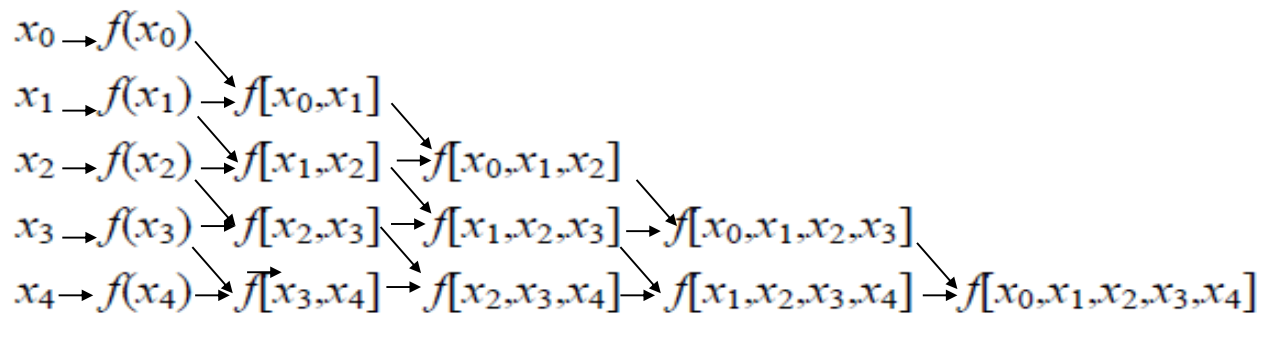
\includegraphics[width=0.7\linewidth]{figs/diff.png}
\end{figure}

将 Taylor 展开式和 Newton 展开式进行推广,可以得到广义 Newton 展开式。从均差的定义可以看出,它的极限与导数有密切关系。事实上,利用罗尔定理可以证明:若 $f(x)$ 在 $[a,b]$ 上存在 $n$ 阶导数,且节点 $x_0,x_1,\ldots,x_n\in[a,b]$,则存在 $\xi\in[a,b]$ 使得:
\[
    f([x_0,x_1,\ldots,x_n])=\frac{f^{(n)}(\xi)}{n!}
\]
因此,我们可以定义在相同点处的“广义”均差为:
\[
    f([c,c,\ldots,c])=\frac{f^{(n)}(c)}{n!}
\]
那么,Taylor 展开就可以看作是广义 Newton 展开在插值节点重合的特殊情形。
广义的均差也可以借助均差表计算,例如:
\begin{figure}[H]
    \centering
    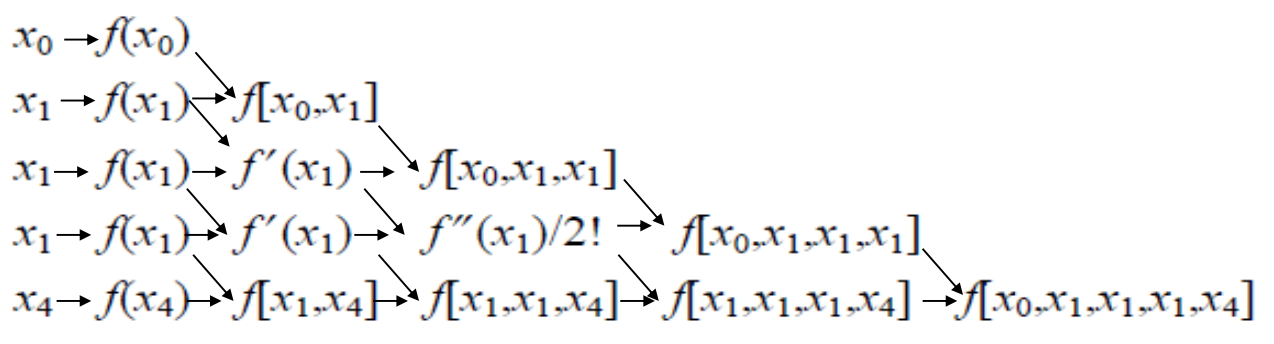
\includegraphics[width=0.7\linewidth]{figs/diff2.png}
\end{figure}

\begin{example}
设 $A=\begin{bmatrix}2&0&0\\1&1&2\\1&-1&3\end{bmatrix}$,求 $e^{At}$.

解:特征方程为:
\[
    \varphi(\lambda)=\begin{vmatrix}\lambda-2&0&0\\-1&\lambda-1&-2\\-1&1&\lambda-3\end{vmatrix}=(\lambda-2)(\lambda-5)(\lambda+1)
\]
画均差表:
\begin{figure}[H]
    \centering
    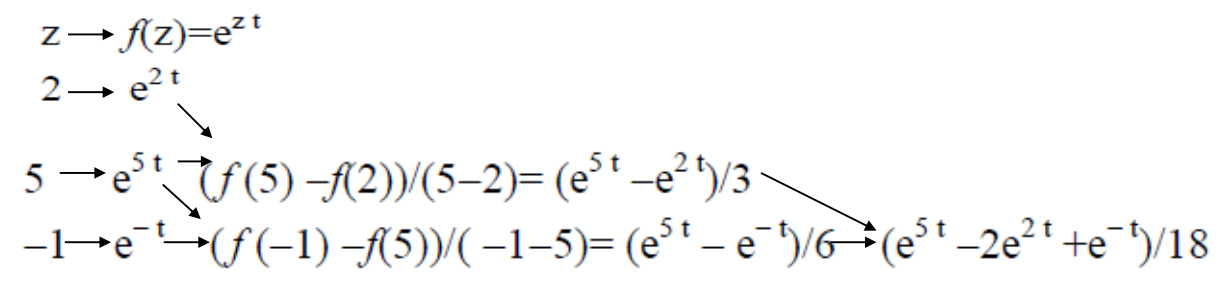
\includegraphics[width=0.7\linewidth]{figs/diff-ex.png}
\end{figure}
于是:
\[
    r(\lambda)=e^{2t}+\frac{e^{5t}-e^{2t}}{3}(\lambda-2)+\frac{e^{5t}-2e^{2t}+e^{-t}}{18}(\lambda-2)(\lambda-5)
\]
故:
\[
    e^{At}=r(A)=\cdots
\]
\end{example}

\paragraph{数项级数求和法}

暂略。



\paragraph{对角形法}

若 $A$ 可对角化,即存在非奇异矩阵 $P$,使得:
\[
    P^{-1}AP=\begin{bmatrix}\lambda_1&&\\&\ddots&\\&&\lambda_n\end{bmatrix}
\]
则:
\[
    f(A)=P\begin{bmatrix}f(\lambda_1)&&\\&\ddots&\\&&f(\lambda_n)\end{bmatrix}P^{-1}
\]

\begin{note}
对角化的计算量较大,因为要计算 $P$ 和 $P^{-1}$,即解特征值和特征向量。
\end{note}


\paragraph{Jordan 标准形法}

在第一章中我们已经推导过了 Jordan 标准形的多项式,而对于一般函数,根据代入规则容易知道其结论有类似的形式。

设 $A$ 的 Jordan 标准形为 $J$,则存在可逆矩阵 $P$ 使得:
\[
    P^{-1}AP=J=\begin{bmatrix}J_1&&\\&\ddots&\\&&J_s\end{bmatrix},\quad J_i=\begin{bmatrix}\lambda_i&1&&\\&\ddots&\ddots&\\&&\lambda_i&1\\&&&\lambda_i\end{bmatrix}_{m_i\times m_i}
\]
那么:
\[
    f(J_i)=\begin{bmatrix}
    f(\lambda_i)&\frac{1}{1!}f'(\lambda_i)&\frac{1}{2!}f''(\lambda_i)&\cdots&\frac{1}{(m_i-1)!}f^{(m_i-1)}(\lambda_i)\\
    &f(\lambda_i)&\frac{1}{1!}f'(\lambda_i)&\cdots&\frac{1}{(m_i-2)!}f^{(m_i-2)}(\lambda_i)\\
    &&\ddots&\ddots&\vdots\\
    &&&f(\lambda_i)&\frac{1}{1!}f'(\lambda_i)\\
    &&&&f(\lambda_i)
    \end{bmatrix}_{m_i\times m_i}
\]
于是原问题:
\[
    f(A)=Pf(J)P^{-1}=P\begin{bmatrix}f(J_1)&&\\&\ddots&\\&&f(J_s)\end{bmatrix}P^{-1}
\]


\subsection{矩阵的微分与积分}

\begin{definition}[矩阵的导数]
若 $A(t)=\left(a_{ij}(t)\right)\in\mathbb C^{m\times n}$ 的每个元素 $a_{ij}(t)$ 都是 $t$ 的可微函数,则 $A(t)$ 关于 $t$ 的导数定义为:
\[
    \frac{\mathrm d}{\mathrm dt}A(t)=A'(t)=\left(a'_{ij}(t)\right)_{m\times n}
\]
\end{definition}
\begin{property}
\[
    \frac{\mathrm d}{\mathrm dt}(A(t)+B(t))=\frac{\mathrm d}{\mathrm dt}A(t)+\frac{\mathrm d}{\mathrm dt}B(t)
\]
\end{property}
\begin{property}
\[
    \frac{\mathrm d}{\mathrm dt}(A(t)B(t))=\frac{\mathrm d}{\mathrm dt}A(t)\cdot B(t)+A(t)\cdot\frac{\mathrm d}{\mathrm dt}B(t)
\]
\end{property}
\begin{corollary}
若 $C(t)=A(t)B(t)$,则:
\[
    \mathrm dC=\mathrm dA\cdot B+A\cdot\mathrm dB
\]
其中,$\mathrm dA=(\mathrm dA/\mathrm dt)\cdot \mathrm dt$,$\mathrm dB=(\mathrm dB/\mathrm dt)\cdot \mathrm dt$.
\end{corollary}

\begin{example}[逆矩阵的导数]
\[
    \frac{\mathrm d}{\mathrm dt}\left(A(t)^{-1}\right)=-A(t)^{-1}\frac{\mathrm dA(t)}{\mathrm dt}A(t)^{-1}
\]
\end{example}
\begin{proof}
由于 $A(t)\cdot A(t)^{-1}=I$,两边求导得:
\[
    \frac{\mathrm d}{\mathrm dt}A(t)\cdot A(t)^{-1}+A(t)\cdot\frac{\mathrm d}{\mathrm dt}\left(A(t)^{-1}\right)=0
\]
故:
\[
    \frac{\mathrm d}{\mathrm dt}\left(A(t)^{-1}\right)=-A(t)^{-1}\frac{\mathrm dA(t)}{\mathrm dt}A(t)^{-1}
\]
\end{proof}

\begin{property}
\[
    \frac{\mathrm d}{\mathrm dt}(\alpha(t)A(t))=\alpha'(t)A(t)+\alpha(t)\cdot\frac{\mathrm d}{\mathrm dt}A(t)
\]
\end{property} 
\begin{property}
若 $A(t)$ 和 $\frac{\mathrm d}{\mathrm dt}A(t)$ \textbf{可交换},$f(z)$ 是与 $t$ 无关的一元解析函数,则:
\[
    \frac{\mathrm d}{\mathrm dt}f(A(t))=f'(A(t))\cdot\frac{\mathrm d}{\mathrm dt}A(t)
\]
\end{property}
\begin{proof}[形式证明(不严格)]
若将 $f(z)$ 展开为幂级数的形式 $f(z)=\sum_{k=0}^\infty c_kz^k$,则根据可交换条件有:
\[
    \frac{\mathrm d}{\mathrm dt}A^k(t)=\sum_{i=0}^{k-1}A^i(t)\cdot\frac{\mathrm d}{\mathrm dt}A(t)\cdot A^{k-1-i}(t)=kA^{k-1}(t)\cdot\frac{\mathrm d}{\mathrm dt}A(t)
\]
代入矩阵函数得:
\[
    \frac{\mathrm d}{\mathrm dt}f(A(t))=\sum_{k=0}^\infty c_k\left(kA^{k-1}(t)\cdot\frac{\mathrm d}{\mathrm dt}A(t)\right)=f'(A(t))\cdot\frac{\mathrm d}{\mathrm dt}A(t)
\]
\end{proof}

\begin{property}[迹函数求导基本定理]
若 $A(t)$ 和 $B(t)$ 可交换,$f(z)$ 是与 $t$ 无关的一元解析函数,则:
\[
    \frac{\mathrm d}{\mathrm dt}\mathrm{tr}\big(f(A(t))\cdot B(t)\big)=\mathrm{tr}\left(f'(A(t))\cdot\frac{\mathrm d}{\mathrm dt}A(t)B(t)\right)+\mathrm{tr}\left(f(A(t))\cdot\frac{\mathrm d}{\mathrm dt}B(t)\right)
\]
\end{property}
\begin{corollary}
取 $B(t)=I$,则有:
\[
    \frac{\mathrm d}{\mathrm dt}\mathrm{tr}(f(A(t)))=\mathrm{tr}\left(f'(A(t))\cdot\frac{\mathrm d}{\mathrm dt}A(t)\right)
\]
\end{corollary}

\begin{definition}[矩阵的积分]
若矩阵 $A(t)=(a_{ij}(t))\in\mathbb C^{m\times n}$ 的每个元素 $a_{ij}(t)$ 都在 $[t_0,t]$ 上可积,则称 $A(t)$ 可积,记为:
\[
    \int_{t_0}^t A(\tau)\mathrm d\tau=\left(\int_{t_0}^ta_{ij}(\tau)\mathrm d\tau\right)_{m\times n}
\]
\end{definition}
\begin{property}
\[
    \int_{t_0}^t[A(\tau)+B(\tau)]\mathrm d\tau=\int_{t_0}^tA(\tau)\mathrm d\tau+\int_{t_0}^tB(\tau)\mathrm d\tau
\]
\end{property}
\begin{property}
\begin{align*}
    &\int_{t_0}^t[A\cdot B(\tau)]\mathrm d\tau=A\cdot\left[\int_{t_0}^tB(\tau)\mathrm d\tau\right]\\
    &\int_{t_0}^t[A(\tau)\cdot B]\mathrm d\tau=\left[\int_{t_0}^tA(\tau)\mathrm d\tau\right]\cdot B
\end{align*}
\end{property}
\begin{property}
\[
    \frac{\mathrm d}{\mathrm dt}\int_{t_0}^tA(\tau)\mathrm d\tau=A(t)
\]
\end{property}
\begin{property}
\[
    \int_{t_0}^{t_1}A'(\tau)\mathrm d\tau=A(t_1)-A(t_0)
\]
\end{property}

\vskip 1cm

前文涉及到的矩阵函数是从矩阵到矩阵的映射,接下来我们探讨关于矩阵各个元素的函数,即从矩阵到数的映射,称作\textbf{函数矩阵}。注意区分函数矩阵与矩阵函数。
为了方便后续推导,首先列出\textbf{矩阵元素与矩阵符号的代数关系式},可以帮助避免将矩阵的各个分量列出来的繁琐。
我们约定 $e_i$ 表示第 $i$ 个分量为 1、其余分量为 0 的单位列向量,其维数由上下文确定,即同一个式子中出现的 $e_i,e_j$ 可能是不同维数的。那么有以下关系式:

\begin{itemize}
    \item 用分量表示矩阵:
    \[
        A=\sum_{i=1}^m\sum_{j=1}^na_{ij}e_ie_j^T
    \]

    \item 用矩阵表示分量:
    \[
        a_{ij}=e_i^TAe_j
    \]

    \item 矩阵逐列拉成向量:
    \[
        \text{Vec}(A)=\sum_{i=1}^m\sum_{j=1}^na_{ij}e_j\otimes e_i=\sum_{i=1}^mA^T e_i\otimes e_i=\sum_{j=1}^ne_j\otimes Ae_j
    \]

    \item 用拉成向量的矩阵表示分量:
    \[
        a_{ij}=(e_j\otimes e_i)^T\text{Vec}(A)
    \]
\end{itemize}

\begin{definition}[函数矩阵的导数]
设 $X=(\xi_{ij})_{m\times n}$,$f(X)$ 为 $mn$ 元函数:
\[
    f(X)=f(\xi_{11},\ldots,\xi_{1n},\xi_{21},\ldots,\xi_{2n},\ldots,\xi_{m1},\ldots,\xi_{mn})
\]
定义 $f(X)$ 对矩阵 $X$ 的导数为:
\[
    \frac{\mathrm df}{\mathrm dX}=\left(\frac{\partial f}{\partial \xi_{ij}}\right)_{m\times n}=
    \begin{bmatrix}
    \dfrac{\partial f}{\partial \xi_{11}}&\cdots&\dfrac{\partial f}{\partial \xi_{1n}}\\
    \vdots&\ddots&\vdots\\
    \dfrac{\partial f}{\partial \xi_{m1}}&\cdots&\dfrac{\partial f}{\partial \xi_{mn}}\\
    \end{bmatrix}
    =\sum_{i=1}^m\sum_{j=1}^n\frac{\partial f}{\partial \xi_{ij}}e_ie_j^T
\]
\end{definition}

\begin{theorem}[函数矩阵的微分形式]
设 $X=(\xi_{ij})_{m\times n}$,$f(X)$ 为 $mn$ 元函数:
\[
    f(X)=f(\xi_{11},\ldots,\xi_{1n},\xi_{21},\ldots,\xi_{2n},\ldots,\xi_{m1},\ldots,\xi_{mn})
\]
则有:
\[
    \frac{\mathrm df}{\mathrm dX}=A\iff \mathrm df=\mathrm{tr}(A^T\cdot\mathrm dX)=\mathrm{tr}(A\cdot \mathrm dX^T)
\]
\end{theorem}
\begin{proof}
\begin{align*}
    \mathrm df&=\sum_{i=1}^m\sum_{j=1}^n\frac{\partial f}{\partial\xi_{ij}}\mathrm d\xi_{ij}\\
    &=\sum_{i=1}^m\sum_{j=1}^n\left(e_i^T\frac{\mathrm df}{\mathrm dX}e_j\right)\left(e_i^T\cdot \mathrm dX\cdot e_j\right)\\
    &=\sum_{i=1}^m\sum_{j=1}^ne_j^T\left(\frac{\mathrm df}{\mathrm dX}\right)^Te_ie_i^T\cdot\mathrm dX\cdot e_j\\
    &=\sum_{j=1}^ne_j^T\left(\frac{\mathrm df}{\mathrm dX}\right)^T\left(\sum_{i=1}^me_ie_i^T\right)\cdot\mathrm dX\cdot e_j\\
    &=\sum_{j=1}^ne_j^T\left(\frac{\mathrm df}{\mathrm dX}\right)^T\mathrm dX\cdot e_j\\
    &=\mathrm{tr}\left(\left(\frac{\mathrm df}{\mathrm dX}\right)^T\mathrm dX\right)\\
    &=\mathrm{tr}(A^T\cdot\mathrm dX)
\end{align*}
\end{proof}

\begin{remark}
上述定理非常重要!!!它告诉我们:\textbf{要求 $\mathrm df/\mathrm dX$,只需要将 $\mathrm df$ 写作形如 $\mathrm{tr}(A^T\mathrm dX)$ 的形式,那么 $A$ 就是结果}。以下所有内容都围绕这一点展开。
\end{remark}

\begin{property}[链式法则]
设 $f(x)$ 是向量 $x$ 的函数,$x$ 是标量 $t$ 的函数 $x=x(t)$,则:
\[
    \frac{\mathrm df}{\mathrm dt}=\frac{\mathrm dx^T}{\mathrm dt}\cdot\frac{\mathrm df}{\mathrm dx}
\]
\end{property}
\begin{property}[链式法则]
设 $f(X)$ 是 $m\times n$ 矩阵 $X$ 各元素的函数,而 $X$ 又是标量 $t$ 的函数,则:
\[
    \frac{\mathrm df}{\mathrm dt}=\mathrm{tr}\left(\frac{\mathrm dX^T}{\mathrm dt}\cdot\frac{\mathrm df}{\mathrm dX}\right)
\]
\end{property}
\begin{proof}
根据微分形式:
\[
    \mathrm df=\mathrm{tr}\left(\left(\frac{\mathrm df}{\mathrm dX}\right)^T\mathrm dX\right),\quad \mathrm dX=\frac{\mathrm dX}{\mathrm dt}\mathrm dt
\]
有:
\[
    \mathrm df=\mathrm{tr}\left(\left(\frac{\mathrm df}{\mathrm dX}\right)^T\frac{\mathrm dX}{\mathrm dt}\mathrm dt\right)=\mathrm{tr}\left(\left(\frac{\mathrm df}{\mathrm dX}\right)^T\frac{\mathrm dX}{\mathrm dt}\right)\mathrm dt=\mathrm{tr}\left(\frac{\mathrm dX^T}{\mathrm dt}\cdot\frac{\mathrm df}{\mathrm dX}\right)\mathrm dt
\]
\end{proof}

\begin{example}[迹函数的导数]
\begin{align*}
    &\frac{\mathrm d}{\mathrm dX}\mathrm{tr}(X^TA)=A\\
    &\frac{\mathrm d}{\mathrm dX}\mathrm{tr}(A^TX)=A\\
    &\frac{\mathrm d}{\mathrm dX}\mathrm{tr}(AX)=A^T
\end{align*}
\end{example}
\begin{proof}
微分是线性算子,可以放入 $\mathrm{tr}(\cdot)$,因此:
\[
    \mathrm d(\mathrm{tr}(X^TA))=\mathrm{tr}(\mathrm d(X^TA))=\mathrm{tr}(\mathrm dX^T A)=\mathrm{tr}(A^T\mathrm dX)
\]
根据微分形式,$\mathrm d(\mathrm{tr}(X^TA))/\mathrm dX=A$.  其他两式类似。证毕。
\end{proof}
\begin{example}
设 $X$ 为可逆矩阵,$f(X)=\mathrm{tr}(AX^{-1})$,则:
\[
    \frac{\mathrm d}{\mathrm dX}f(X)=-(X^{-1}AX^{-1})^T
\]
\end{example}
\begin{proof}
\[
    \mathrm df(X)=\mathrm{tr}(\mathrm d(AX^{-1}))=\mathrm{tr}(A\cdot\mathrm dX^{-1})
\]
由于 $XX^{-1}=I$,两边取微分得:$\mathrm dX\cdot X^{-1}+X\cdot\mathrm dX^{-1}=0$,故 $\mathrm dX^{-1}=-X^{-1}\cdot\mathrm dX\cdot X^{-1}$,因此:
\[
    \mathrm df(X)=\mathrm{tr}\left(A\cdot(-X^{-1}\mathrm dX X^{-1})\right)=\mathrm{tr}\left((-X^{-1}AX^{-1})\mathrm dX\right)
\]
根据微分形式,$\mathrm df(X)/\mathrm dX=(-X^{-1}AX^{-1})^T$.
\end{proof}

\begin{example}
设 $f(x)=x^TAx$,则:
\[
    \frac{\mathrm df}{\mathrm dx}=(A+A^T)x
\]
\end{example}
\begin{proof}
\begin{align*}
    \mathrm df&=\mathrm d(x^TAx)=\mathrm dx^TAx+x^TA\mathrm dx=x^T A^T\mathrm dx+x^TA\mathrm dx\\&=x^T(A^T+A)\mathrm dx=\mathrm{tr}\left(((A+A^T)x)^T\cdot\mathrm dx\right)
\end{align*}
根据微分形式,$\mathrm df/\mathrm dx=(A+A^T)x$.
\end{proof}

\begin{example}
更多迹函数求导结论:
\begin{figure}[H]
    \centering
    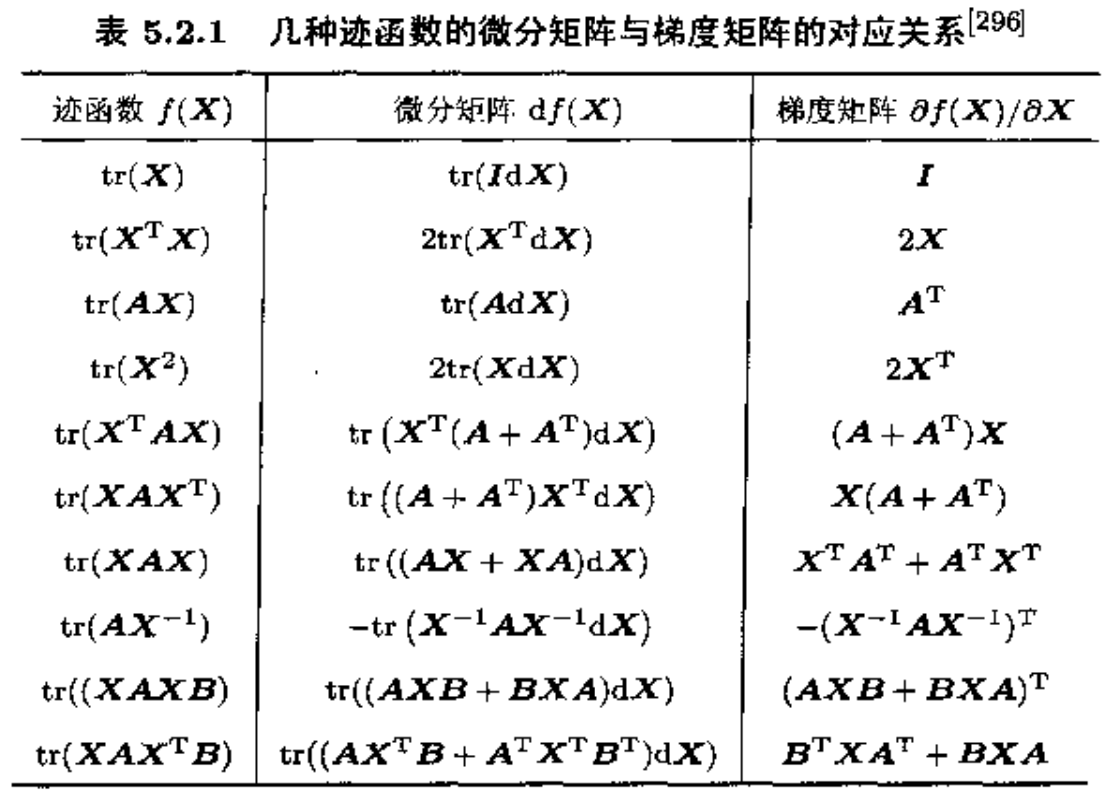
\includegraphics[width=0.7\linewidth]{figs/table1.png}
\end{figure}
\end{example}

\begin{example}[行列式求导]
设矩阵 $X$ 非奇异,则:
\[
    \frac{\mathrm d(|X|)}{\mathrm dX}=|X|(X^{-1})^T
\]
或有微分形式:
\[
    \mathrm d|X|=|X|\mathrm{tr}(X^{-1}\mathrm dX)=\mathrm{tr}(|X|X^{-1}\mathrm dX)
\]
\end{example}
\begin{proof}
设 $c_{ij}$ 为 $x_{ij}$ 的代数余子式,根据行列式定义知:
\[
    |X|=\sum_{i=1}^nc_{ij}x_{ij},\quad\forall j
\]
由于 $c_{ij}$ 与 $x_{ij}$ 无关,所以有 $\partial|X|/\partial x_{ij}=c_{ij}$,于是有微分:
\[
    \mathrm d|X|=\sum_{i=1}^n\sum_{j=1}^n c_{ij}\mathrm dx_{ij}=\mathrm{tr}(X^\ast\mathrm dX)
\]
其中 $X^\ast$ 是 $X$ 的伴随矩阵,由于 $X^\ast=|X|X^{-1}$,因此:
\[
    \mathrm d|X|=\mathrm{tr}(|X|X^{-1}\mathrm dX)
\]
\end{proof}

\begin{example}
对于任意非奇异矩阵 $X$,有:
\[
    \frac{\mathrm d(\ln|X|)}{\mathrm dX}=(X^T)^{-1}
\]
\end{example}
\begin{example}
对于任意 $X\in\mathbb R^{m\times n}$,
\[
    \frac{\mathrm d(\ln|\delta I+X^TX|)}{\mathrm dX}=2X(\delta I+X^TX)
\]
其中 $\delta$ 是与矩阵 $A$ 无关的常数。
\end{example}
\begin{example}
更多行列式求导结论:
\begin{figure}[H]
    \centering
    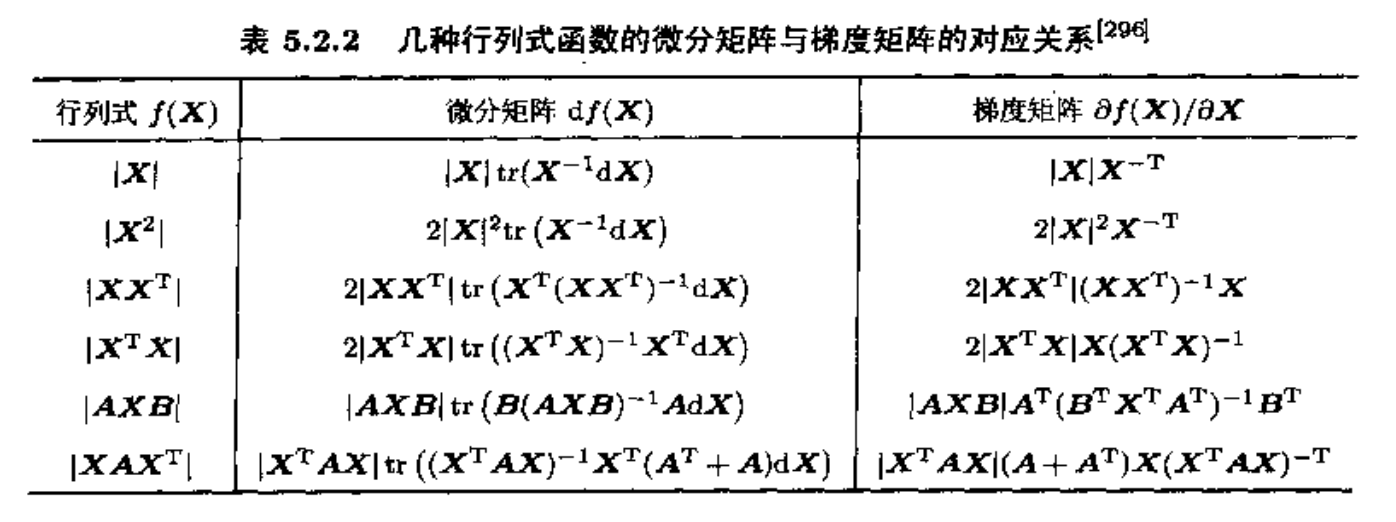
\includegraphics[width=0.9\linewidth]{figs/table2.png}
\end{figure}
\end{example}

\begin{definition}[直积 / Kronecker 积]
设 $A\in\mathbb C^{m\times n},\,B\in\mathbb C^{p\times q}$,称如下分块矩阵为 $A$ 与 $B$ 的直积:
\[
    A\otimes B=\begin{bmatrix}a_{11}B&a_{12}B&\cdots&a_{1n}B\\a_{21}B&a_{22}B&\cdots&a_{2n}B\\\vdots&\vdots&\ddots&\vdots\\a_{m1}B&a_{m2}B&\cdots&a_{mn}B\\\end{bmatrix}\in\mathbb C^{mp\times nq}
\]
特别地,若 $A\in\mathbb C^{m\times 1},\,B\in\mathbb C^{n\times 1}$,则 $A\otimes B^T=AB^T$.
\end{definition}

\begin{definition}[矩阵函数对矩阵的导数]
设有关于 $X=(\xi_{ij})_{m\times n}$ 的 $mn$ 元函数:
\[
    f_{ij}(X)=f_{ij}(\xi_{11},\ldots,\xi_{1n},\ldots,\xi_{m1},\ldots,\xi_{mn}),\quad i=1,\ldots,r,\,j=1,\ldots,s
\]
定义矩阵:
\[
    F(X)=\begin{bmatrix}f_{11}&\cdots&f_{1s}\\\vdots&\ddots&\vdots\\f_{r1}&\cdots&f_{rs}\end{bmatrix}
\]
定义 $F(X)$ 的导数如下:
\[
    \frac{\mathrm dF}{\mathrm dX}=
    \begin{bmatrix}
    \dfrac{\partial F}{\partial \xi_{11}}&\cdots&\dfrac{\partial F}{\partial \xi_{1n}}\\
    \vdots&\ddots&\vdots\\
    \dfrac{\partial F}{\partial \xi_{m1}}&\cdots&\dfrac{\partial F}{\partial \xi_{mn}}
    \end{bmatrix}=\sum_{i=1}^m\sum_{j=1}^n(e_ie_j^T)\otimes\frac{\partial F}{\partial \xi_{ij}}
\]
其中,
\[
    \frac{\partial F}{\partial \xi_{ij}}=
    \begin{bmatrix}
    \dfrac{\partial f_{11}}{\partial \xi_{ij}}&\cdots&\dfrac{\partial f_{1s}}{\partial \xi_{ij}}\\
    \vdots&\ddots&\vdots\\
    \dfrac{\partial f_{r1}}{\partial \xi_{ij}}&\cdots&\dfrac{\partial f_{rs}}{\partial \xi_{ij}}
    \end{bmatrix}=\sum_{k=1}^r\sum_{l=1}^s\frac{\partial f_{kl}}{\partial \xi_{ij}}e_ke_l^T
\]
特别地,当 $F\in\mathbb C^{m\times 1}$ 且 $X\in\mathbb C^{n\times 1}$ 时,
\[
    \frac{\mathrm dF}{\mathrm dX^T}=
    \begin{bmatrix}
    \dfrac{\partial f_{1}}{\partial \xi_{1}}&\cdots&\dfrac{\partial f_{1}}{\partial \xi_{n}}\\
    \vdots&\ddots&\vdots\\
    \dfrac{\partial f_{m}}{\partial \xi_{1}}&\cdots&\dfrac{\partial f_{m}}{\partial \xi_{n}}
    \end{bmatrix}
\]
即 Jacobian 矩阵。
\end{definition}

\begin{property}[链式法则]
设 $f(x)$ 是向量 $x$ 的函数,$x$ 又是 $u$ 的函数,则:
\[
    \frac{\mathrm df}{\mathrm du}=\frac{\mathrm dx^T}{\mathrm du}\frac{\mathrm df}{\mathrm dx}
\]
\end{property}

\begin{theorem}[向量函数关于向量导数的微分形式]
设 $y=F(x)$ 是向量 $x$ 的向量值函数,则:
\[
    \frac{\mathrm dy}{\mathrm dx^T}=A\iff\mathrm dy=A\mathrm dx
\]
\end{theorem}
\begin{note}
一些论文中可能会把 $\mathrm dy/\mathrm dx^T$ 不严谨地直接写作 $\mathrm dy/\mathrm dx$.
\end{note}

\begin{example}[在微分方程中的应用]
考虑微分方程:
\[
    \begin{cases}
    x_1'(t)=a_{11}x_1(t)+a_{12}x_2(t)+\cdots+a_{1n}x_n(t)+b_1(t)\\
    x_2'(t)=a_{21}x_1(t)+a_{22}x_2(t)+\cdots+a_{2n}x_n(t)+b_2(t)\\
    \quad\vdots\\
    x_n'(t)=a_{n1}x_1(t)+a_{n2}x_2(t)+\cdots+a_{nn}x_n(t)+b_n(t)\\
    \end{cases}
\]
令:
\[
    A=\begin{bmatrix}a_{11}&\cdots&a_{1n}\\\vdots&\ddots&\vdots\\a_{n1}&\cdots&a_{nn}\end{bmatrix},\quad
x(t)=\begin{bmatrix}x_1(t)\\\vdots\\x_n(t)\end{bmatrix},\quad
b(t)=\begin{bmatrix}b_1(t)\\\vdots\\b_n(t)\end{bmatrix}
\]
则可写作矩阵形式:
\[
    x'(t)=A\cdot x(t)+b(t)
\]
\end{example}

\begin{theorem}
齐次微分方程 $x'(t)=Ax(t)$ 的通解为:
\[
    x(t)=e^{tA}c
\]
其中 $c$ 为任意常向量。若再加上初始条件 $x(t_0)=x_0$,则解为:
\[
    x(t)=e^{(t-t_0)A}x_0
\]
\end{theorem}

\begin{theorem}
非齐次微分方程 $x'(t)=Ax(t)+b(t)$ 的通解为:
\[
    x(t)=x_1(t)+x_2(t)
\]
其中 $x_1(t)=e^{tA}c$ 是对应齐次微分方程的通解,$x_2(t)$ 是非齐次微分方程的一个特解。常向量 $c$ 由初始条件确定。特解可使用\textbf{常数变易法}计算得到:设 $x_2(t)=e^{tA}c(t)$,代入原非齐次微分方程有:
\[
    e^{tA}c'(t)=b(t)
\]
由此可以解出一个 $c(t)$,从而得到一个特解。
\end{theorem}
